% ===========================================================================
% OS/161 Assignment 2 - Implementation Report
%
% Brief: "Please go through the Assignment document and implement the system
%         calls. Also implement basic file system calls, including create,
%         read, write, append, etc."
%
% NOTE: LaTeX SOURCE only -- not compiled here.
% Build later (from inside the assignment2/ folder):  pdflatex assignment2-report.tex
% Screenshots are read from ./SS/ (relative to this file).
% ===========================================================================
\documentclass[11pt,a4paper]{article}

\usepackage[utf8]{inputenc}
\usepackage[T1]{fontenc}
\usepackage[margin=1in]{geometry}
\usepackage{graphicx}
\usepackage{xcolor}
\usepackage{listings}
\usepackage{booktabs}
\usepackage{longtable}
\usepackage{array}
\usepackage{caption}
\usepackage{subcaption}
\usepackage{enumitem}
\usepackage{placeins}   % \FloatBarrier -- keeps figures inside their section
\usepackage{float}      % [H] placement specifier
\usepackage{hyperref}

\hypersetup{
    colorlinks=true,
    linkcolor=blue!55!black,
    urlcolor=blue!55!black,
    citecolor=blue!55!black
}

% Tighter, consistent captions.
\captionsetup{font=small,labelfont=bf,skip=6pt}
\setlist{itemsep=2pt,topsep=3pt}

% ---- Code listing style ---------------------------------------------------
\definecolor{codebg}{gray}{0.97}
\definecolor{codekw}{rgb}{0.10,0.10,0.60}
\definecolor{codecomment}{rgb}{0.00,0.45,0.00}
\definecolor{codestr}{rgb}{0.60,0.10,0.10}

\lstdefinestyle{code}{
    backgroundcolor=\color{codebg},
    basicstyle=\ttfamily\footnotesize,
    keywordstyle=\color{codekw}\bfseries,
    commentstyle=\color{codecomment}\itshape,
    stringstyle=\color{codestr},
    numbers=none,
    frame=single,
    framesep=5pt,
    rulecolor=\color{gray!40},
    breaklines=true,
    showstringspaces=false,
    tabsize=4,
    captionpos=b,
    aboveskip=8pt,
    belowskip=8pt
}
\lstset{style=code}

% -------------------------------------------------
% Helper commands
% -------------------------------------------------
\newcommand{\coursecode}{CSE 3211}
\newcommand{\coursename}{Operating Systems Lab}
\newcommand{\reporttitle}{OS/161 --- Assignment 2}
\newcommand{\studentname}{H.M. Mehedi Hasan}
\newcommand{\studentroll}{13}
\newcommand{\session}{2022--2023}
\newcommand{\submissiondate}{13/07/2026}

% ---- Title ----------------------------------------------------------------
 
\date{}

\begin{document}
% -------------------------------------------------
% Cover Page - black-and-white format
% -------------------------------------------------
\begin{titlepage}
\thispagestyle{empty}
\begin{center}
\vspace*{1.1cm}

{\Large\bfseries 3rd Year 2nd Semester}\\[0.55cm]
{\Large\bfseries University of Dhaka}\\[0.35cm]
{\large\bfseries Department of Computer Science and Engineering}\\[0.35cm]
{\large Session: \session}\\[1.4cm]

\rule{0.78\textwidth}{0.8pt}\\[0.65cm]
{\Large\bfseries \coursecode: \coursename}\\[1.0cm]

{\Huge\bfseries Lab Report}\\[0.45cm]
{\Large\bfseries \reporttitle}\\[0.65cm]
\rule{0.78\textwidth}{0.8pt}\\[1.4cm]
  

{\large\bfseries Submission Date:}\\[0.2cm]
{\large \submissiondate}\\[1.2cm]

{\large\bfseries Submitted By:}\\[0.25cm]
{\large\bfseries \studentname}\\[0.2cm]
{\large Roll: \studentroll}

\vfill
\end{center}
\end{titlepage}

\pagenumbering{roman}
\tableofcontents
\newpage
\pagenumbering{arabic}

 

% ===========================================================================
\section{Objective}
% =======================================================================

\begin{enumerate}[leftmargin=1.4em]
  \item \textbf{Process system calls:} \texttt{fork}, \texttt{execv},
        \texttt{waitpid}, \texttt{getpid}, \texttt{\_exit}.
  \item \textbf{File-system system calls} on a per-process file-descriptor
        table: \texttt{open}, \texttt{close}, \texttt{read}, \texttt{write},
        \texttt{lseek}, \texttt{dup2}, plus the directory/metadata calls.
  \item \textbf{Basic file operations} built on those syscalls ---
        \emph{create}, \emph{read}, \emph{write}, \emph{append}, \emph{copy}.
\end{enumerate}

% ===========================================================================
\section{Architecture at a Glance}
% ===========================================================================
A user program calls a libc wrapper, which traps into the kernel dispatcher.
The dispatcher resolves the file descriptor through the per-process table and
issues a \texttt{VOP\_*} operation to the file system.

\begin{lstlisting}[caption={End-to-end path of a file operation.}]
 userland      file_rwc, fileoperations, /bin/ls, /bin/cat ...
    |          libc wrapper: open(), read(), write(), remove() ...
    v
 syscall layer            src/kern/syscall/file_syscalls.c
    |   sys_open / sys_read / sys_write / sys_close / sys_lseek ...
    v
 FD table                 src/kern/proc/proc.c , include/proc.h
    |   openfile{ of_vnode, of_offset, of_flags, of_refcount }
    v
 SFS file system          src/kern/fs/sfs/*.c   (fileops/dirops/linkops)
    |
    v
 disk image (SFS)   or   emufs (host pass-through)
\end{lstlisting}

Process syscalls follow a parallel path through \texttt{process\_syscalls.c}
backed by a small PID table in \texttt{proc.c}.

\FloatBarrier
% ===========================================================================
\section{Process-Control System Calls}
% ===========================================================================
Previously the shell died with \texttt{fork: Function not implemented}
(\texttt{SYS\_fork} is syscall 0). The following were added.

\paragraph{Process state (\texttt{include/proc.h}).}
Each \texttt{struct proc} gained a PID, parent pointer, exit state, and a wait
semaphore (\texttt{p\_pid}, \texttt{p\_parent}, \texttt{p\_exited},
\texttt{p\_exitstatus}, \texttt{p\_waitsem}).

\paragraph{PID table + helpers (\texttt{proc/proc.c}).}
A fixed table (\texttt{PID\_MAX = 128}) backs registration and lookup, with
helpers \texttt{proc\_allocpid}, \texttt{proc\_register},
\texttt{proc\_create\_fork}, \texttt{proc\_exit}, \texttt{proc\_wait}.

\paragraph{Syscalls (\texttt{syscall/process\_syscalls.c}).}
\begin{itemize}[leftmargin=1.4em]
  \item \texttt{sys\_fork} --- copy trapframe + address space, create a child
        with its own PID; parent gets the child PID, child returns 0.
  \item \texttt{sys\_execv} --- copy path + \texttt{argv} into the kernel, load
        the executable, rebuild \texttt{argv} on the new stack, then
        \texttt{enter\_new\_process}.
  \item \texttt{sys\_waitpid} --- block on the child's \texttt{p\_waitsem}, then
        return the encoded status.
  \item \texttt{sys\_getpid} --- return \texttt{curproc->p\_pid}.
\end{itemize}

The child returns from \texttt{fork} in \texttt{enter\_forked\_process}
(\texttt{arch/mips/syscall/syscall.c}):

\begin{lstlisting}[language=C,caption={Forked-child return: v0 = 0, then step past the syscall.}]
void
enter_forked_process(void *data1, unsigned long unused)
{
    struct trapframe *tf = data1, childtf;
    (void)unused;
    memcpy(&childtf, tf, sizeof(childtf));
    kfree(tf);
    childtf.tf_v0 = 0;      /* child sees fork() == 0   */
    childtf.tf_a3 = 0;      /* no error                 */
    childtf.tf_epc += 4;    /* step over syscall instr. */
    mips_usermode(&childtf);
    panic("mips_usermode returned\n");
}
\end{lstlisting}

\paragraph{Supporting changes.}
\texttt{menu.c} now calls \texttt{proc\_wait} after launching a program, so the
child owns the console until it exits. For the low-RAM DUMBVM setup,
\texttt{execv} copies arguments per-argument (instead of a fixed 64\,KB
\texttt{ARG\_MAX} buffer) and \texttt{DUMBVM\_STACKPAGES} was cut from 18 to 4,
letting \texttt{fork}+\texttt{execv} fit.

\FloatBarrier
% ===========================================================================
\section{Console I/O and the File-Descriptor Table}
% ===========================================================================
\texttt{console\_syscalls.c} exposes \texttt{console\_read}/\texttt{console\_write}
helpers. Descriptors 0/1/2 route through them; all others go through the
per-process FD table --- so \texttt{printf}/\texttt{scanf} keep working while
real files use the FS path.

\begin{lstlisting}[language=C,caption={Open-file object and per-process FD table.}]
struct openfile {
    struct vnode *of_vnode;    /* underlying file           */
    off_t         of_offset;   /* current file pointer      */
    int           of_flags;    /* O_RDONLY/O_WRONLY/O_APPEND */
    int           of_refcount; /* shared via dup2           */
};
struct fdarray { struct openfile *fd_table[FD_MAX]; };  /* FD_MAX = 32 */
\end{lstlisting}

Reference-counting helpers keep it correct: \texttt{fdalloc} (lowest free slot),
\texttt{fdget}, \texttt{of\_release} (free at refcount 0), \texttt{fdclose}.
\texttt{dup2} shares one \texttt{openfile} across slots; \texttt{proc\_exit}
calls \texttt{fd\_destroy\_all} so no vnode leaks.

\FloatBarrier
% ===========================================================================
\section{File-System System Calls}
% ===========================================================================
All file syscalls live in \texttt{syscall/file\_syscalls.c}, dispatched from
\texttt{arch/mips/syscall/syscall.c}.

\begin{longtable}{@{}l l l@{}}
\caption{File-system system calls and their kernel path.}\label{tab:syscalls}\\
\toprule
\textbf{Syscall} & \textbf{Entry point} & \textbf{Kernel path} \\
\midrule
\endfirsthead
\multicolumn{3}{c}{\tablename~\thetable\ (continued)}\\
\toprule
\textbf{Syscall} & \textbf{Entry point} & \textbf{Kernel path} \\
\midrule
\endhead
\bottomrule
\endfoot
\texttt{open}       & \texttt{sys\_open}      & \texttt{vfs\_open} $\to$ \texttt{fdalloc} \\
\texttt{close}      & \texttt{sys\_close}     & \texttt{fdclose} $\to$ \texttt{of\_release} \\
\texttt{read}       & \texttt{sys\_read}      & \texttt{fd\_io} $\to$ \texttt{VOP\_READ} \\
\texttt{write}      & \texttt{sys\_write}     & \texttt{fd\_io} $\to$ \texttt{VOP\_WRITE} \\
\texttt{lseek}      & \texttt{sys\_lseek}     & offset arithmetic on \texttt{openfile} \\
\texttt{dup2}       & \texttt{sys\_dup2}      & share \texttt{openfile} between slots \\
\texttt{chdir}      & \texttt{sys\_chdir}     & update \texttt{curproc->p\_cwd} \\
\texttt{\_\_getcwd} & \texttt{sys\_\_\_getcwd}& \texttt{vfs\_getcwd} / \texttt{sfs\_namefile} \\
\texttt{mkdir}      & \texttt{sys\_mkdir}     & \texttt{vfs\_mkdir} \\
\texttt{rmdir}      & \texttt{sys\_rmdir}     & \texttt{vfs\_rmdir} \\
\texttt{link}       & \texttt{sys\_link}      & hardlink creation \\
\texttt{remove}     & \texttt{sys\_unlink}    & \texttt{vfs\_remove} \\
\texttt{symlink}    & \texttt{sys\_symlink}   & \texttt{sfs\_symlink} (new inode) \\
\texttt{readlink}   & \texttt{sys\_readlink}  & \texttt{sfs\_readlink} \\
\texttt{fstat}      & \texttt{sys\_fstat}     & \texttt{VOP\_STAT} on FD's vnode \\
\texttt{stat}       & \texttt{sys\_stat}      & \texttt{vfs\_lookup} + \texttt{VOP\_STAT} \\
\texttt{lstat}      & \texttt{sys\_lstat}     & same path as \texttt{stat} \\
\end{longtable}

\FloatBarrier
% ===========================================================================
\section{The Basic File Operations}
% ===========================================================================
The four required operations (plus \emph{copy}) are expressed directly on the
syscalls above.

\begin{table}[H]
\centering
\caption{Basic file operations and their mechanism.}\label{tab:ops}
\begin{tabular}{@{}l l l@{}}
\toprule
\textbf{Operation} & \textbf{Expressed as} & \textbf{Mechanism} \\
\midrule
create & \texttt{open(O\_WRONLY|O\_CREAT|O\_TRUNC)} & new inode via \texttt{vfs\_open} \\
write  & \texttt{write(fd, buf, n)}                 & \texttt{fd\_io} $\to$ \texttt{VOP\_WRITE} \\
read   & \texttt{read(fd, buf, n)}                  & \texttt{fd\_io} $\to$ \texttt{VOP\_READ} \\
append & \texttt{open(\dots\,|\,O\_APPEND)}         & \texttt{of\_offset} $\gets$ EOF via \texttt{VOP\_STAT} \\
copy   & \texttt{read} + \texttt{write} loop        & both via the FD table \\
\bottomrule
\end{tabular}
\end{table}

\noindent\textbf{Append.} On \texttt{open} with \texttt{O\_APPEND}, the kernel
reads the current size via \texttt{VOP\_STAT} and sets
\texttt{of\_offset = st\_size}, so every write lands at end-of-file.

\FloatBarrier
%  ===========================================================================
\section{Files Modified / Added}
% ===========================================================================
\begin{longtable}{@{}l l@{}}
\caption{Files touched for Assignment 2.}\label{tab:files}\\
\toprule
\textbf{File} & \textbf{Change} \\
\midrule
\endfirsthead
\multicolumn{2}{c}{\tablename~\thetable\ (continued)}\\
\toprule
\textbf{File} & \textbf{Change} \\
\midrule
\endhead
\bottomrule
\endfoot
\multicolumn{2}{@{}l}{\emph{Process / threads}}\\
\texttt{kern/include/proc.h}              & process + FD state, helper decls \\
\texttt{kern/proc/proc.c}                 & PID table, fork/exit/wait, FD helpers \\
\texttt{kern/thread/thread.c}             & wake waiter on thread exit \\
\texttt{kern/syscall/process\_syscalls.c} & \emph{(new)} fork/execv/waitpid/getpid \\
\texttt{kern/main/menu.c}                 & wait on launched program \\
\texttt{kern/arch/mips/vm/dumbvm.c}       & stack pages 18 $\to$ 4 \\
\addlinespace
\multicolumn{2}{@{}l}{\emph{File-system syscalls}}\\
\texttt{kern/syscall/file\_syscalls.c}    & \emph{(new)} all file syscalls \\
\texttt{kern/syscall/console\_syscalls.c} & console\_read/write helpers \\
\texttt{kern/include/syscall.h}           & prototypes \\
\texttt{kern/arch/mips/syscall/syscall.c} & dispatcher cases, forked-child entry \\
\addlinespace
\multicolumn{2}{@{}l}{\emph{SFS}}\\
\texttt{kern/fs/sfs/sfs\_vnops.c}         & symlink/readlink/getdirentry/stat \\
\texttt{kern/fs/sfs/sfs\_inode.c}         & \texttt{SFS\_TYPE\_LINK} dispatch \\
\texttt{kern/fs/sfs/sfsprivate.h}         & \texttt{sfs\_linkops} decl \\
\texttt{kern/include/kern/sfs.h}          & \texttt{SFS\_TYPE\_LINK = 3} \\
\addlinespace
\multicolumn{2}{@{}l}{\emph{Userland / build}}\\
\texttt{userland/lib/libc/unix/fileops.c} & \emph{(new)} libc wrappers \\
\texttt{userland/testbin/file\_rwc/}      & \emph{(new)} rwc + append test \\
\texttt{userland/testbin/fileoperations/} & \emph{(new)} write/cat/append/copy \\
\texttt{userland/testbin/file\_link/}     & \emph{(new)} symlink test \\
\texttt{kern/conf/conf.kern}              & compile the new syscall files \\
 
\end{longtable}

\FloatBarrier
% ===========================================================================
\section{Build and Run}
% ===========================================================================
\begin{lstlisting}[language=bash,caption={From the Ubuntu WSL shell.}]
cd  OSLab/polito_os161/os161
./build.sh all      # kernel + userland (first time)
./build.sh kernel   # incremental, after a kernel edit
./run-os161.sh      # boot System/161
\end{lstlisting}

\FloatBarrier
% ===========================================================================
\section{Results}
% ===========================================================================
Every feature was verified live in System/161. Screenshots are in
\texttt{assignment2/SS/}.

% ---- Process syscalls -----------------------------------------------------
\subsection{Process syscalls --- argument passing}
\begin{figure}[H]
\centering
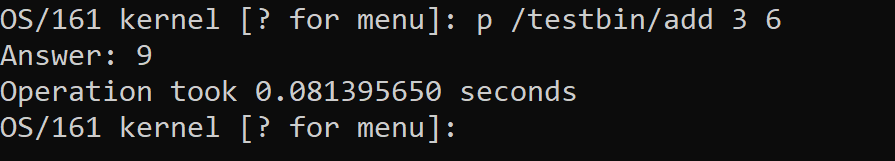
\includegraphics[width=0.68\textwidth]{SS/arg_pass.PNG}
\caption{\texttt{p /testbin/add 3 6} $\to$ \texttt{Answer: 9}: \texttt{fork} +
         \texttt{execv} pass \texttt{argc}/\texttt{argv} correctly.}
\end{figure}

\textbf{Explanation of Output:} The screenshot above shows the \texttt{add} user program being executed with arguments "3" and "6". The \texttt{fork} + \texttt{execv} system calls successfully pass \texttt{argc} and \texttt{argv} into the new process's address space. This allows the program to read the arguments, compute their sum, and correctly output "9".

\begin{figure}[H]
\centering
\begin{subfigure}{0.48\textwidth}
  \centering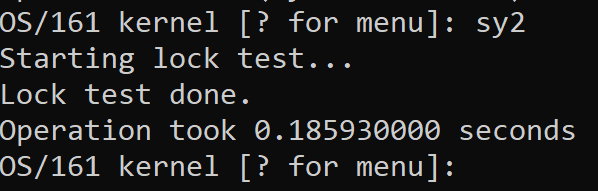
\includegraphics[width=\linewidth]{SS/sy2.PNG}
  \caption{\texttt{sy2} --- lock test passes.}
\end{subfigure}\hfill
\begin{subfigure}{0.48\textwidth}
  \centering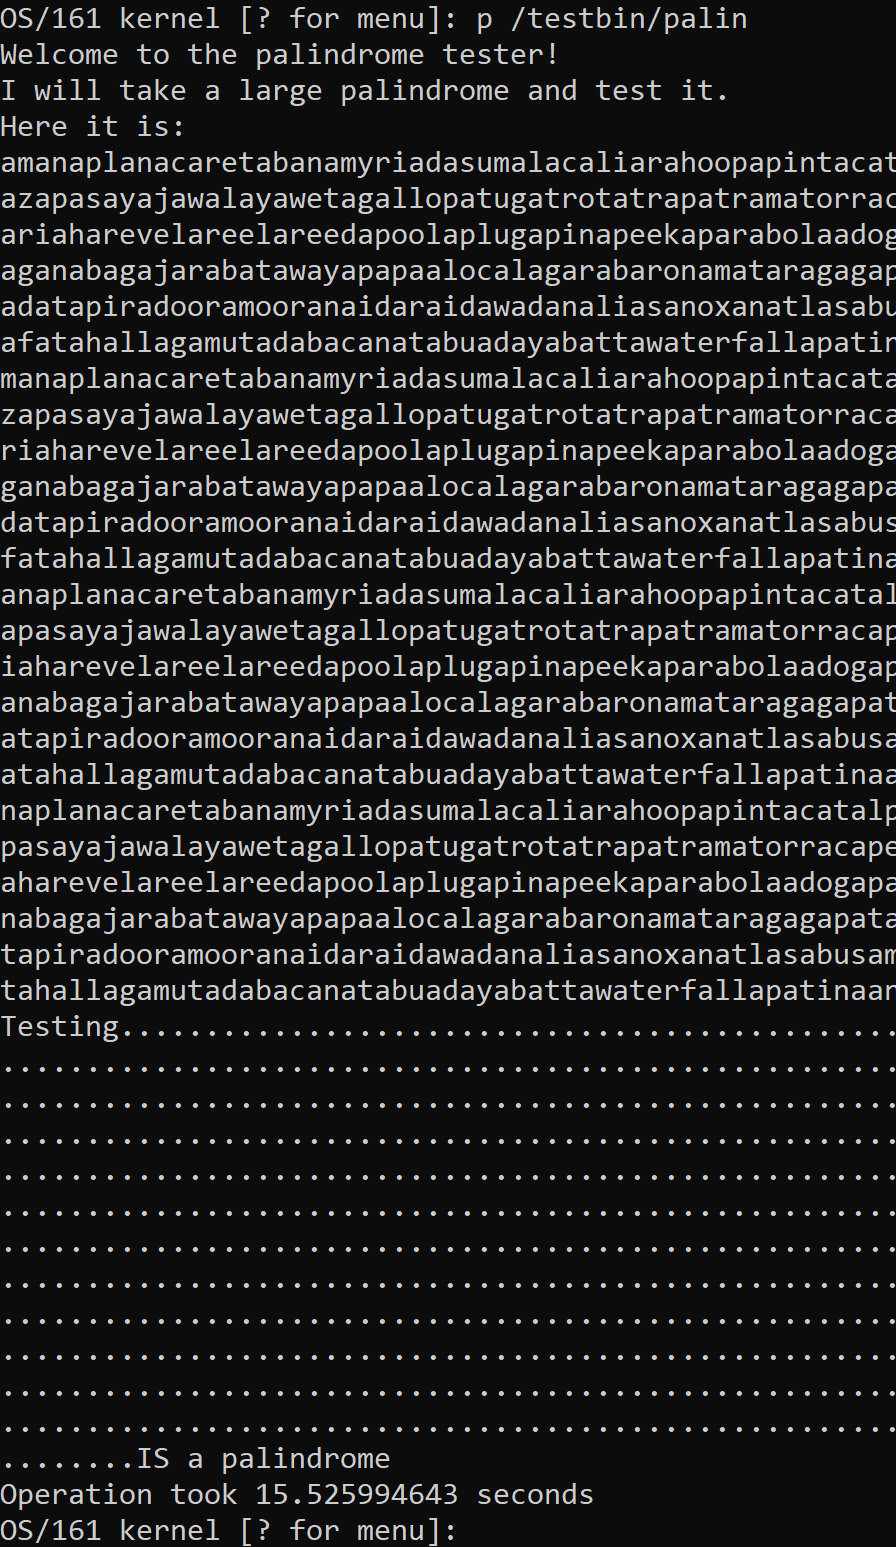
\includegraphics[width=\linewidth]{SS/palin.PNG}
  \caption{Another program via fork/execv.}
\end{subfigure}
\caption{Synchronization sanity check and an additional program run.}
\end{figure}

\textbf{Explanation of Output:} 
\begin{itemize}[leftmargin=1.4em]
    \item \textbf{sy2:} This output proves that our process and file system additions did not break the kernel's basic thread synchronization primitives. The lock test completes successfully.
    \item \textbf{palin:} This output shows that computationally intensive programs (like checking for palindromes) load and execute properly via our \texttt{execv} implementation without memory corruption.
\end{itemize}

\begin{figure}[H]
\centering
\begin{subfigure}{0.48\textwidth}
  \centering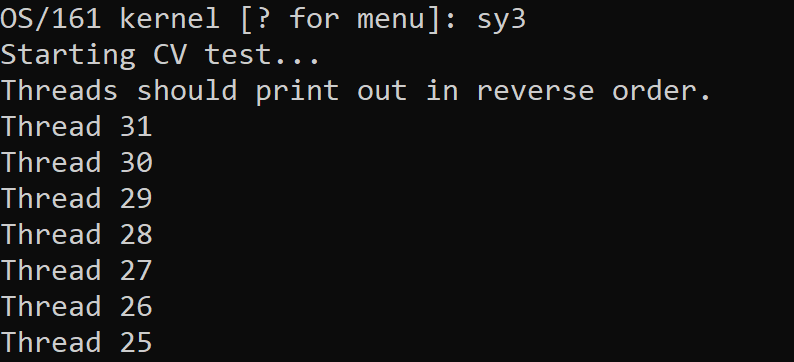
\includegraphics[width=\linewidth]{SS/sy3a.PNG}
  \caption{Threads start printing in reverse order (31, 30, 29, \dots).}
\end{subfigure}\hfill
\begin{subfigure}{0.48\textwidth}
  \centering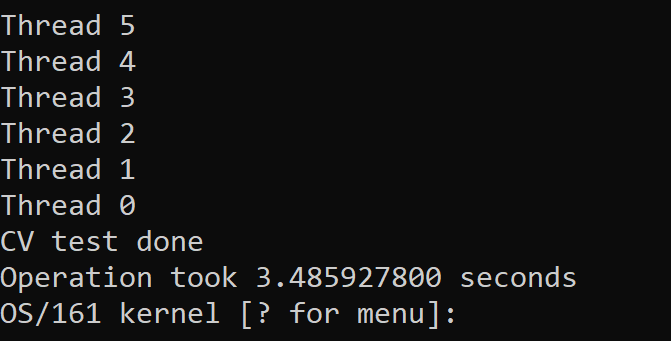
\includegraphics[width=\linewidth]{SS/sy3b.PNG}
  \caption{\dots down to Thread 0, then ``CV test done''.}
\end{subfigure}
\caption{\texttt{sy3} --- condition-variable test: threads print in strict
         reverse order, confirming correct CV signalling.}
\end{figure}

\textbf{Explanation of Output:} The screenshots show the \texttt{sy3} test. Multiple threads are spawned, but they must use condition variables to coordinate and print in strict reverse order (from 31 down to 0). The output correctly shows this countdown, confirming that CV signalling and wait queues are functioning as expected.

\FloatBarrier
% ---- File operations ------------------------------------------------------
\subsection{Basic file operations}

\begin{figure}[H]
\centering
\begin{subfigure}{0.48\textwidth}
  \centering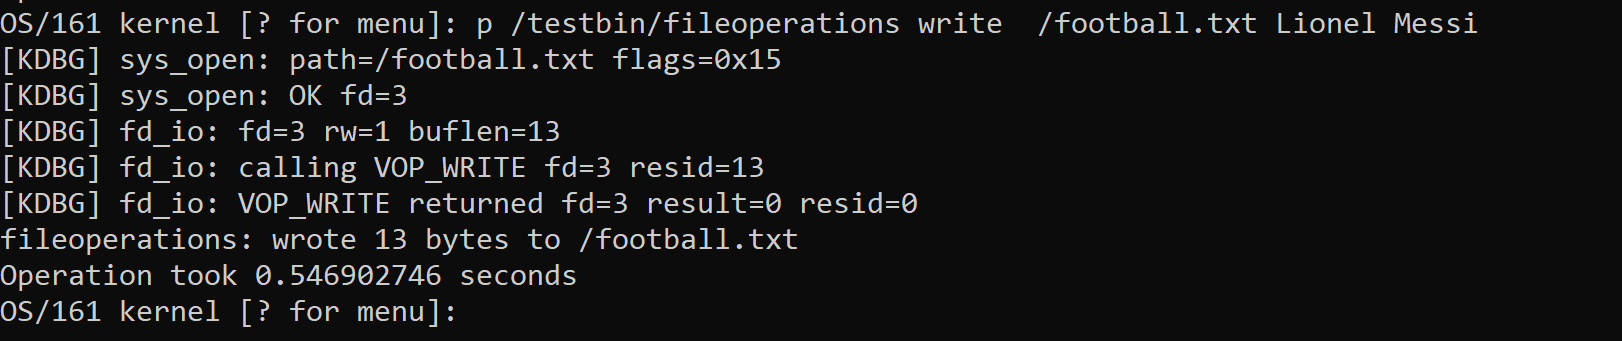
\includegraphics[width=\linewidth]{SS/write.PNG}
  \caption{\textbf{create + write} --- \texttt{flags=0x15}
           (\texttt{O\_WRONLY|O\_CREAT|O\_TRUNC}), then \texttt{VOP\_WRITE}.}
\end{subfigure}\hfill
\begin{subfigure}{0.48\textwidth}
  \centering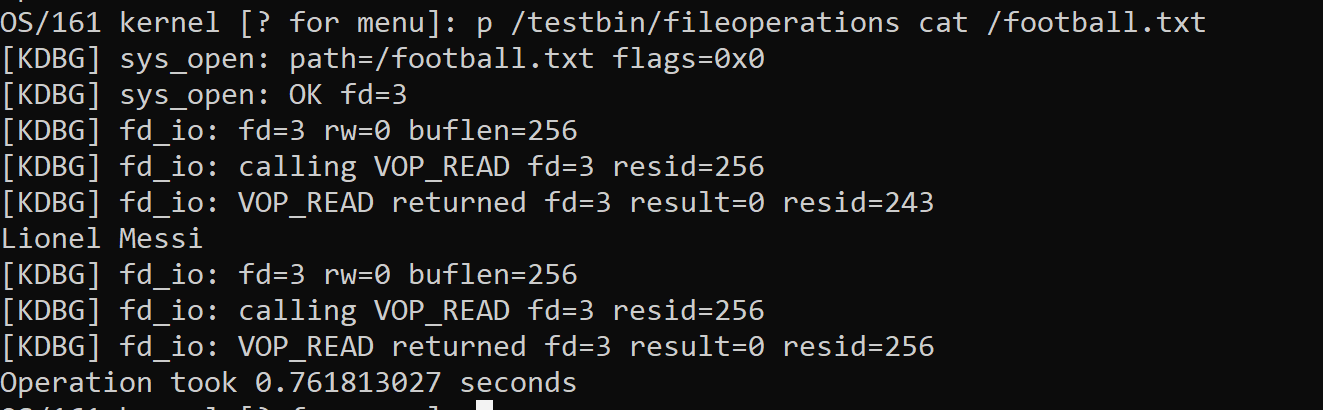
\includegraphics[width=\linewidth]{SS/read.PNG}
  \caption{\textbf{read} --- \texttt{cat /football.txt} $\to$
           \texttt{Lionel Messi} via \texttt{VOP\_READ}.}
\end{subfigure}

\vspace{8pt}

\begin{subfigure}{0.48\textwidth}
  \centering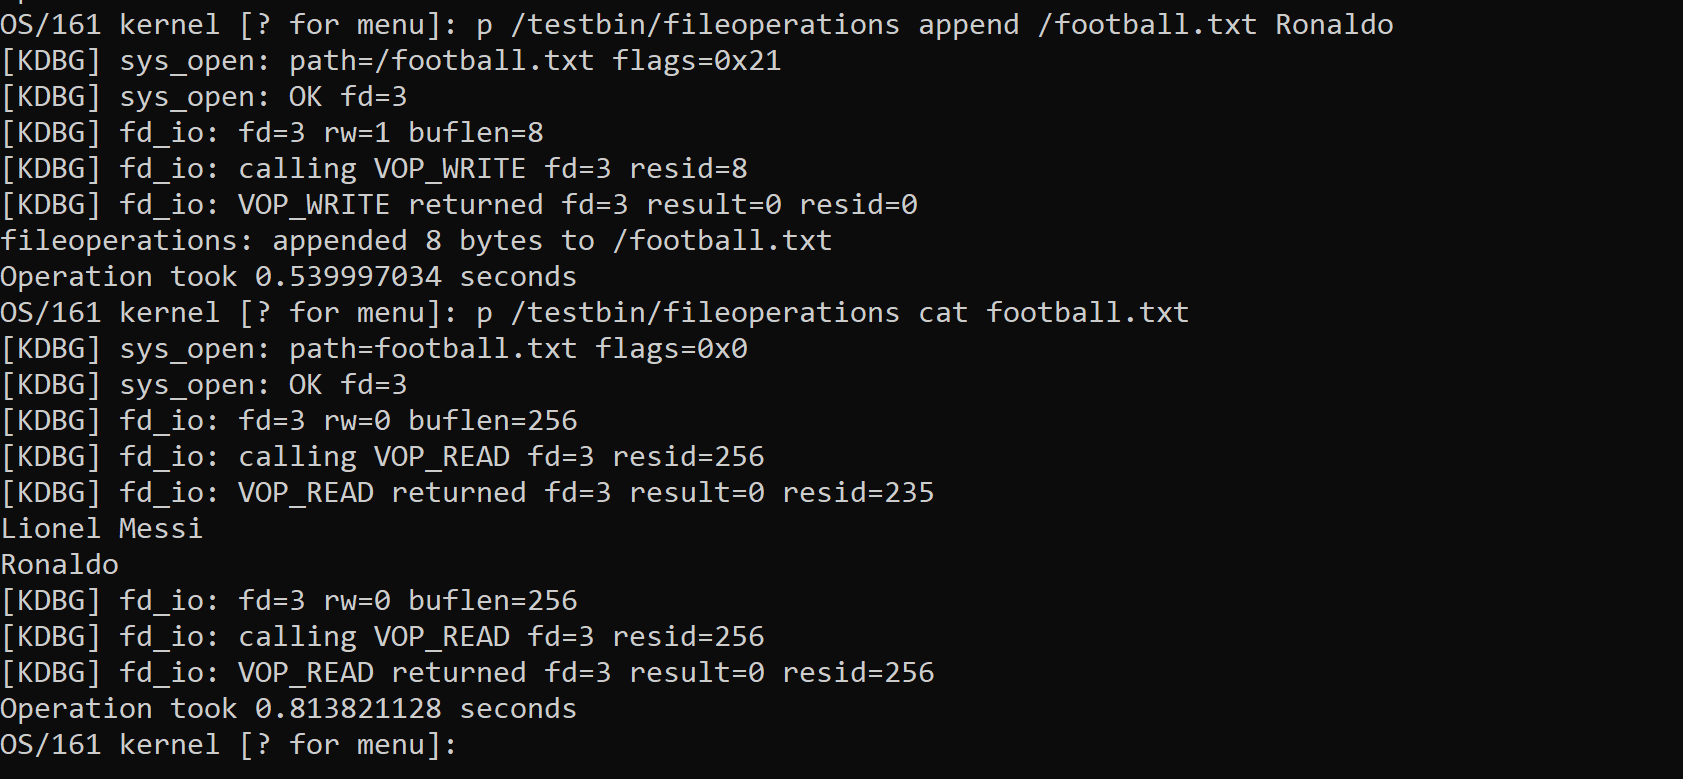
\includegraphics[width=\linewidth]{SS/append.PNG}
  \caption{\textbf{append} --- \texttt{O\_APPEND} (\texttt{flags=0x21}); the
           file now holds \texttt{Messi} \emph{then} \texttt{Ronaldo}.}
\end{subfigure}\hfill
\begin{subfigure}{0.48\textwidth}
  \centering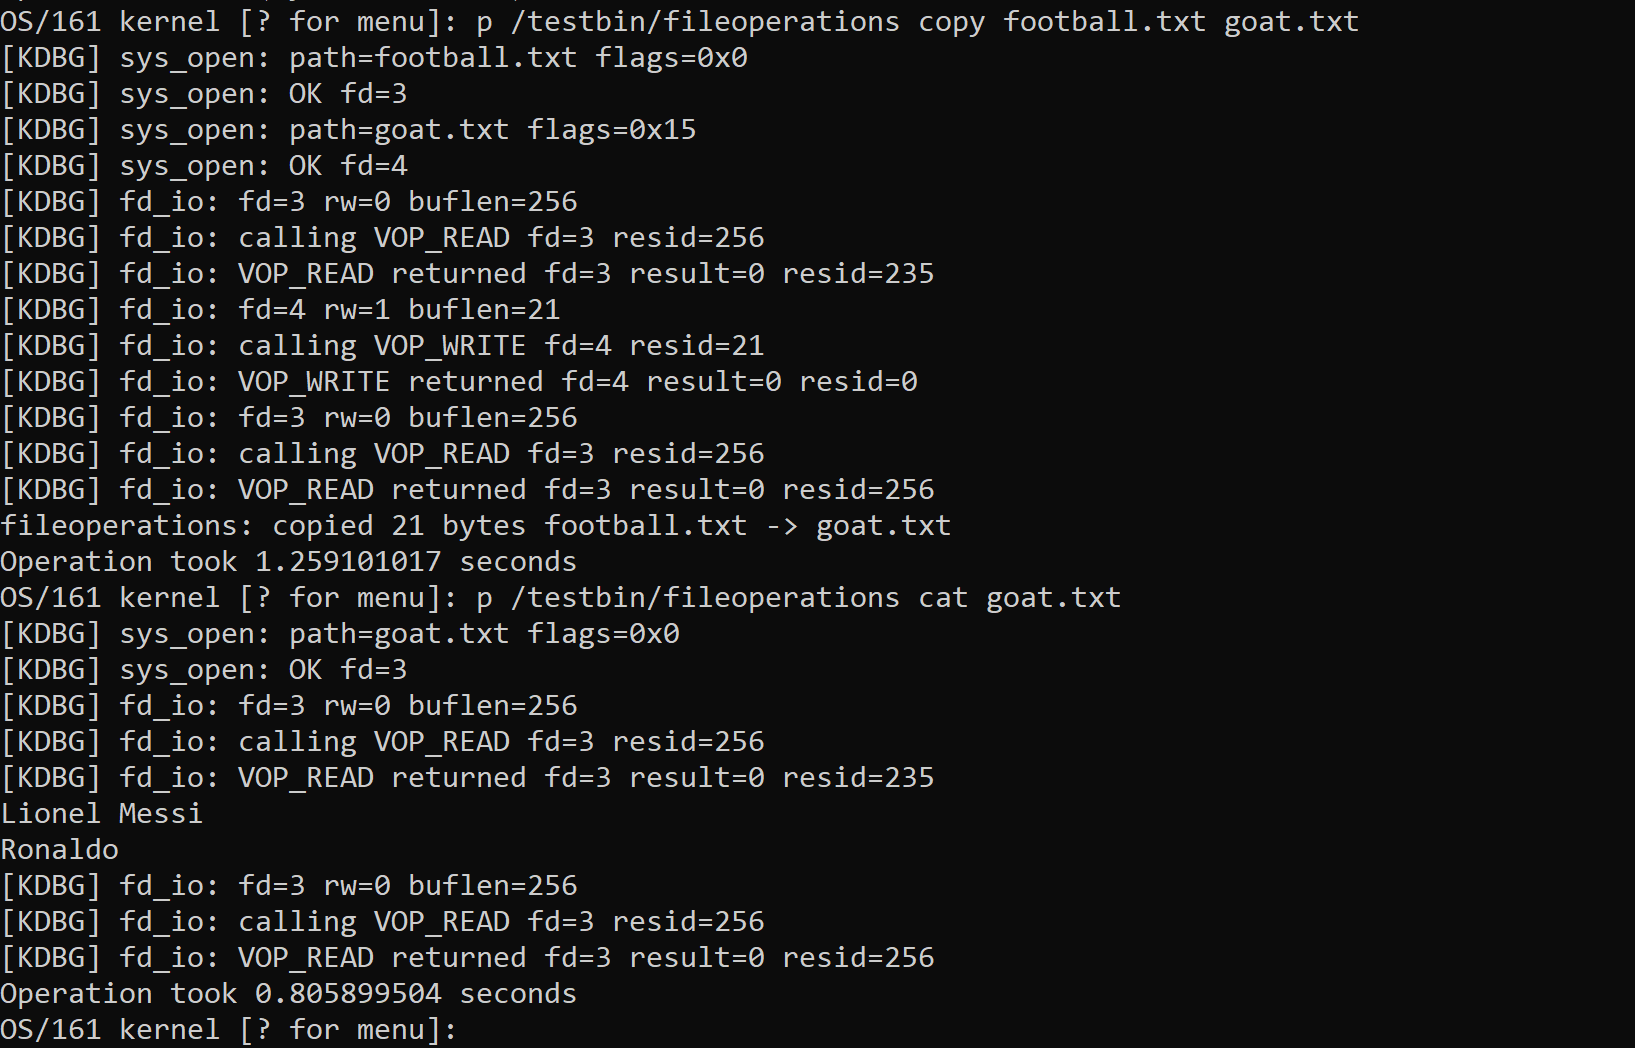
\includegraphics[width=\linewidth]{SS/copy.PNG}
  \caption{\textbf{copy} --- a read/write loop copies 21 bytes
           \texttt{football.txt} $\to$ \texttt{goat.txt}.}
\end{subfigure}
\caption{The four basic file operations demonstrated end-to-end.}
\label{fig:fileops}
\end{figure}

\textbf{Explanation of Output:} 
\begin{itemize}[leftmargin=1.4em]
    \item \textbf{Create + Write (a):} We successfully open a file with \texttt{O\_CREAT} and write data to it. The system correctly allocates an inode and saves the data to the SFS disk.
    \item \textbf{Read (b):} Reading the newly created file using the \texttt{cat} utility outputs exactly what was written earlier, proving that \texttt{sys\_read} properly interfaces with \texttt{VOP\_READ}.
    \item \textbf{Append (c):} When opening a file with the \texttt{O\_APPEND} flag, the kernel correctly seeks to the End-of-File before writing. The output shows new text added after the old text without overwriting it.
    \item \textbf{Copy (d):} The \texttt{copy} utility reads bytes from one file descriptor and writes them to another. The success message confirms that the per-process FD table correctly maintains independent offsets and handles simultaneous reads and writes across different files.
\end{itemize}

\FloatBarrier
% ---- filetest -------------------------------------------------------------
\subsection{\texttt{filetest} --- open / write / read / remove}
\begin{figure}[H]
\centering
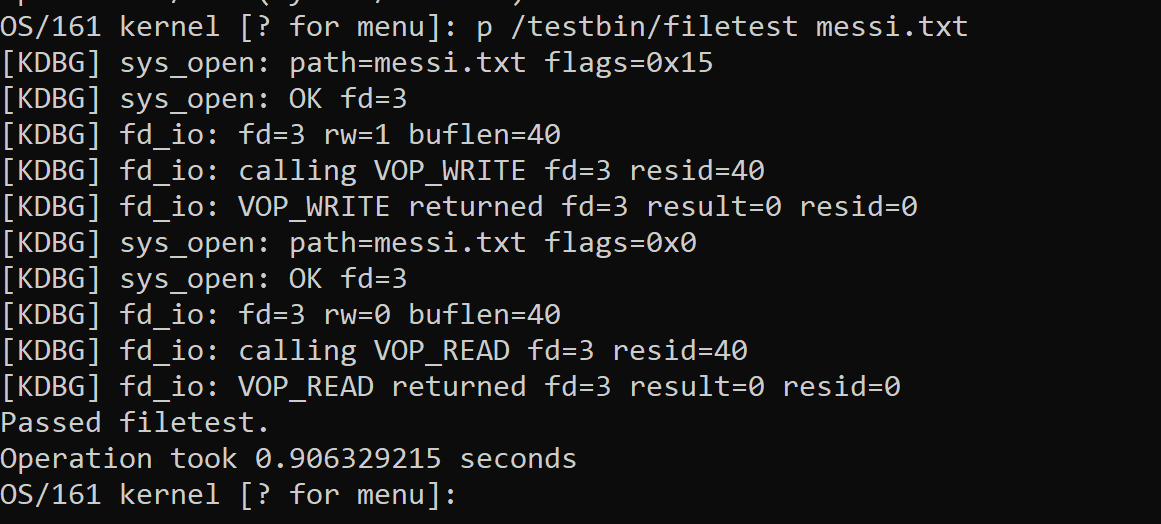
\includegraphics[width=0.80\textwidth]{SS/filetest.PNG}
\caption{\texttt{p /testbin/filetest messi.txt} runs to completion.}
\end{figure}

\textbf{Explanation of Output:} The \texttt{filetest} program issues a series of basic file operations (open, write, read, close) and finishes by removing the file. The output shows a clean run to completion, proving that the file system syscalls are robust.

\FloatBarrier
% ===========================================================================
 

% ===========================================================================
\section{Conclusion}
% ===========================================================================
All Assignment 2 system calls were implemented --- the process-control group
(\texttt{fork}, \texttt{execv}, \texttt{waitpid}, \texttt{getpid},
\texttt{\_exit}), the console path, and the full file-system group on a
per-process file-descriptor table. On top of these, the basic file operations
--- \emph{create}, \emph{read}, \emph{write}, \emph{append}, \emph{copy} ---
were demonstrated end-to-end in System/161 (Figure~\ref{fig:fileops}).

\newpage
% ===========================================================================
\section{Appendix: Source Code}
% ===========================================================================
This appendix contains excerpts of the most important C source files
implemented or modified for Assignment~2.  The code is grouped by
component: process system calls, process table management, file-system
system calls, and userland test programs.

% -------------------------------------------------------------------
\subsection{Data Structures --- \texttt{kern/include/proc.h}}
% -------------------------------------------------------------------
This header defines the core data structures that every other file
depends on: the per-file \texttt{openfile} object, the per-process
file-descriptor table, and the \texttt{proc} structure itself.

\begin{lstlisting}[language=C,
  caption={\texttt{openfile}, \texttt{fdarray}, and \texttt{struct proc}
           --- the data structures added for Assignment~2.}]
struct openfile {
	struct vnode *of_vnode;   /* the vnode for this open file        */
	off_t of_offset;          /* current file position               */
	int of_flags;             /* O_RDONLY / O_WRONLY / O_APPEND etc.  */
	int of_refcount;          /* fd table entries pointing here       */
};

#define FD_MAX 32
struct fdarray {
	struct openfile *fd_table[FD_MAX];
};

struct proc {
	char *p_name;              /* Name of this process             */
	struct spinlock p_lock;    /* Lock for this structure           */
	unsigned p_numthreads;     /* Number of threads                */

	/* VM */
	struct addrspace *p_addrspace;

	/* VFS */
	struct vnode *p_cwd;       /* current working directory         */
	struct fdarray p_fdtable;  /* file descriptor table             */

	/* Process identity and parent/child state */
	pid_t p_pid;
	struct proc *p_parent;
	bool p_exited;
	bool p_waited;
	int p_exitstatus;
	struct semaphore *p_waitsem;
};
\end{lstlisting}

\FloatBarrier
\newpage
% -------------------------------------------------------------------
\subsection{Process System Calls ---
            \texttt{kern/syscall/process\_syscalls.c}}
% -------------------------------------------------------------------
This kernel file implements the process-control system calls
(\texttt{fork}, \texttt{execv}, \texttt{waitpid}, \texttt{getpid}).

\begin{lstlisting}[language=C,
  caption={\texttt{sys\_fork} --- duplicate the trapframe and address
           space, then create a child thread.}]
int sys_fork(struct trapframe *tf, int32_t *retval)
{
	struct trapframe *childtf;
	struct addrspace *childas;
	struct proc *childproc;
	int result;

	childtf = kmalloc(sizeof(*childtf));
	if (childtf == NULL) return ENOMEM;
	memcpy(childtf, tf, sizeof(*childtf));

	result = as_copy(proc_getas(), &childas);
	if (result) {
		kfree(childtf);
		return result;
	}

	childproc = proc_create_fork(curproc->p_name, curproc, childas);
	if (childproc == NULL) {
		as_destroy(childas);
		kfree(childtf);
		return ENOMEM;
	}

	result = thread_fork(curthread->t_name, childproc,
	                     enter_forked_process, childtf, 0);
	if (result) {
		proc_destroy(childproc);
		kfree(childtf);
		return result;
	}

	*retval = childproc->p_pid;   /* parent gets child PID */
	return 0;
}
\end{lstlisting}

\begin{lstlisting}[language=C,
  caption={\texttt{sys\_execv} --- replace the current address space
           with a new executable image.}]
int sys_execv(const_userptr_t progname, userptr_t uargv)
{
	char *kprog;
	char **argv;
	struct addrspace *oldas, *newas;
	struct vnode *v;
	vaddr_t entrypoint, stackptr;
	userptr_t argv_userptr;
	int argc, result;

	if (progname == NULL || uargv == NULL) return EFAULT;

	kprog = kmalloc(PATH_MAX);
	if (kprog == NULL) return ENOMEM;

	result = copyinstr(progname, kprog, PATH_MAX, NULL);
	if (result) { kfree(kprog); return result; }

	result = copyin_args(uargv, &argv, &argc);
	if (result) { kfree(kprog); return result; }

	result = vfs_open(kprog, O_RDONLY, 0, &v);
	if (result) {
		free_args(argv, argc); kfree(kprog); return result;
	}

	newas = as_create();
	if (newas == NULL) {
		vfs_close(v); free_args(argv, argc);
		kfree(kprog); return ENOMEM;
	}

	oldas = proc_setas(newas);
	as_activate();

	result = load_elf(v, &entrypoint);
	vfs_close(v);
	if (result) {
		proc_setas(oldas); as_activate();
		as_destroy(newas); free_args(argv, argc);
		kfree(kprog); return result;
	}

	result = as_define_stack(newas, &stackptr);
	if (result) {
		proc_setas(oldas); as_activate();
		as_destroy(newas); free_args(argv, argc);
		kfree(kprog); return result;
	}

	result = copyout_args(argv, argc, &stackptr, &argv_userptr);
	if (result) {
		proc_setas(oldas); as_activate();
		as_destroy(newas); free_args(argv, argc);
		kfree(kprog); return result;
	}

	as_destroy(oldas);
	free_args(argv, argc);
	kfree(kprog);

	enter_new_process(argc, argv_userptr, NULL,
	                  stackptr, entrypoint);
	panic("enter_new_process returned\n");
	return EINVAL;
}
\end{lstlisting}

\FloatBarrier
\newpage
% -------------------------------------------------------------------
\subsection{Process Table and Lifecycle ---
            \texttt{kern/proc/proc.c}}
% -------------------------------------------------------------------
This file manages the global PID table, process creation/destruction,
file-descriptor helpers, and the \texttt{waitpid} back-end.

\begin{lstlisting}[language=C,
  caption={\texttt{proc\_wait} --- block until the child exits and
           return its encoded status.}]
int proc_wait(pid_t pid, userptr_t statusptr,
              int options, int32_t *retval)
{
	struct proc *child;
	int status, result;
	bool exited;

	if ((options & ~WALLFLAGS) != 0) return EINVAL;
	if (pid <= 0 || pid >= PROC_PID_MAX) return ECHILD;

	spinlock_acquire(&proctable_lock);
	child = proctable[pid];
	if (child == NULL || child->p_parent != curproc
	    || child->p_waited) {
		spinlock_release(&proctable_lock);
		return ECHILD;
	}

	spinlock_acquire(&child->p_lock);
	exited = child->p_exited;
	if (!exited && options == WNOHANG) {
		spinlock_release(&child->p_lock);
		spinlock_release(&proctable_lock);
		if (retval != NULL) *retval = 0;
		return 0;
	}
	child->p_waited = true;
	spinlock_release(&child->p_lock);
	spinlock_release(&proctable_lock);

	if (!exited) {
		P(child->p_waitsem);     /* block until child exits */
	}

	spinlock_acquire(&child->p_lock);
	status = child->p_exitstatus;
	spinlock_release(&child->p_lock);

	if (statusptr != NULL) {
		result = copyout(&status, statusptr, sizeof(status));
		if (result) return result;
	}

	if (retval != NULL) *retval = pid;
	proc_destroy(child);
	return 0;
}
\end{lstlisting}

\begin{lstlisting}[language=C,
  caption={\texttt{proc\_exit} --- mark the process as exited and
           release all file descriptors.}]
void proc_exit(int status)
{
	struct proc *proc = curproc;

	if (proc == NULL) {
		thread_exit();
	}

	/* Release all file descriptors held by this process. */
	fd_destroy_all(proc);

	spinlock_acquire(&proc->p_lock);
	proc->p_exitstatus = _MKWAIT_EXIT(status & 0xff);
	proc->p_exited = true;
	spinlock_release(&proc->p_lock);
}
\end{lstlisting}

\begin{lstlisting}[language=C,
  caption={\texttt{fdalloc} / \texttt{fdget} --- allocate the lowest
           free slot and look up an existing slot.}]
int fdalloc(struct proc *proc, struct openfile *of, int *retval)
{
	int fd;

	/* fds 0-2 are reserved for console I/O; start at 3 */
	for (fd = 3; fd < FD_MAX; fd++) {
		if (proc->p_fdtable.fd_table[fd] == NULL) {
			proc->p_fdtable.fd_table[fd] = of;
			*retval = fd;
			return 0;
		}
	}
	return EMFILE;
}

int fdget(struct proc *proc, int fd, struct openfile **ret)
{
	struct openfile *of;

	if (fd < 0 || fd >= FD_MAX) return EBADF;
	of = proc->p_fdtable.fd_table[fd];
	if (of == NULL) return EBADF;
	of->of_refcount++;
	*ret = of;
	return 0;
}
\end{lstlisting}

\FloatBarrier
\newpage
% -------------------------------------------------------------------
\subsection{Syscall Dispatcher ---
            \texttt{kern/arch/mips/syscall/syscall.c}}
% -------------------------------------------------------------------
The MIPS trap handler calls this dispatcher.  Each \texttt{SYS\_*}
constant is mapped to the corresponding kernel function.

\begin{lstlisting}[language=C,
  caption={Syscall dispatch switch (excerpt) and
           \texttt{enter\_forked\_process}.}]
void syscall(struct trapframe *tf)
{
	int callno;
	int32_t retval = 0;
	int err;

	callno = tf->tf_v0;

	switch (callno) {
	    case SYS_fork:
		err = sys_fork(tf, &retval);  break;
	    case SYS_execv:
		err = sys_execv((const_userptr_t)tf->tf_a0,
		                (userptr_t)tf->tf_a1);  break;
	    case SYS_waitpid:
		err = sys_waitpid((pid_t)tf->tf_a0,
		    (userptr_t)tf->tf_a1,
		    (int)tf->tf_a2, &retval);  break;
	    case SYS_getpid:
		err = sys_getpid(&retval);  break;
	    case SYS__exit:
		sys__exit(tf->tf_a0);
		panic("sys__exit returned\n");  break;
	    case SYS_read:
		err = sys_read((int)tf->tf_a0,
		    (userptr_t)tf->tf_a1,
		    (size_t)tf->tf_a2, &retval);  break;
	    case SYS_write:
		err = sys_write((int)tf->tf_a0,
		    (const_userptr_t)tf->tf_a1,
		    (size_t)tf->tf_a2, &retval);  break;
	    case SYS_open:
		err = sys_open((const_userptr_t)tf->tf_a0,
		    (int)tf->tf_a1,
		    (mode_t)tf->tf_a2, &retval);  break;
	    case SYS_close:
		err = sys_close((int)tf->tf_a0, &retval);  break;
	    /* ... lseek, dup2, chdir, getcwd, mkdir, rmdir,
	     *     link, remove, symlink, readlink,
	     *     fstat, stat, lstat, getdirentry ... */
	    default:
		kprintf("Unknown syscall %d\n", callno);
		err = ENOSYS;  break;
	}

	/* On success: v0 = retval, a3 = 0.
	   On error:   v0 = errno,  a3 = 1. */
	if (err) {
		tf->tf_v0 = err;
		tf->tf_a3 = 1;
	} else {
		tf->tf_v0 = retval;
		tf->tf_a3 = 0;
	}
	tf->tf_epc += 4;   /* advance past syscall instruction */
}

void enter_forked_process(void *data1, unsigned long unused)
{
	struct trapframe *tf = data1, childtf;
	(void)unused;
	memcpy(&childtf, tf, sizeof(childtf));
	kfree(tf);
	childtf.tf_v0 = 0;     /* child sees fork() == 0   */
	childtf.tf_a3 = 0;     /* no error                 */
	childtf.tf_epc += 4;   /* step over syscall instr. */
	mips_usermode(&childtf);
	panic("mips_usermode returned\n");
}
\end{lstlisting}

\FloatBarrier
\newpage
% -------------------------------------------------------------------
\subsection{Console I/O ---
            \texttt{kern/syscall/console\_syscalls.c}}
% -------------------------------------------------------------------
This file provides the backing helpers for file descriptors 0, 1, and 2
(stdin / stdout / stderr), plus \texttt{sys\_\_exit}.

\begin{lstlisting}[language=C,
  caption={\texttt{console\_write}, \texttt{console\_read}, and
           \texttt{sys\_\_exit}.}]
int console_write(const_userptr_t buf, size_t nbytes,
                  int32_t *retval)
{
	char kbuf[CONSOLE_IO_CHUNK];
	size_t done = 0, chunk, i;
	int result;

	while (done < nbytes) {
		chunk = nbytes - done;
		if (chunk > sizeof(kbuf)) chunk = sizeof(kbuf);

		result = copyin((const_userptr_t)((vaddr_t)buf + done),
		                kbuf, chunk);
		if (result) return result;

		for (i = 0; i < chunk; i++) {
			if (kbuf[i] == '\n') putch('\r');
			putch(kbuf[i]);
		}
		done += chunk;
	}
	*retval = (int32_t)done;
	return 0;
}

int console_read(userptr_t buf, size_t buflen,
                 int32_t *retval)
{
	size_t done = 0;
	char ch;
	int result;

	while (done < buflen) {
		ch = getch();
		if (ch == '\r') ch = '\n';

		result = copyout(&ch,
		    (userptr_t)((vaddr_t)buf + done), 1);
		if (result) return result;

		done++;
		if (ch == '\n') break;
	}
	*retval = (int32_t)done;
	return 0;
}

void sys__exit(int code)
{
	proc_exit(code);
	thread_exit();
}
\end{lstlisting}

\FloatBarrier
\newpage
% -------------------------------------------------------------------
\subsection{File-System System Calls ---
            \texttt{kern/syscall/file\_syscalls.c}}
% -------------------------------------------------------------------
All file-related system calls live in this file.

\begin{lstlisting}[language=C,
  caption={\texttt{sys\_open} --- resolve path, allocate an openfile,
           and handle \texttt{O\_APPEND}.}]
int sys_open(const_userptr_t upath, int flags,
             mode_t mode, int32_t *retval)
{
	char *path;
	struct vnode *vn;
	struct openfile *of;
	int result, fd;
	(void)mode;

	if (flags < 0) return EINVAL;

	result = copyin_string(upath, &path, PATH_MAX);
	if (result) return result;

	result = vfs_open(path, flags, mode, &vn);
	if (result) { kfree(path); return result; }

	of = openfile_alloc(vn, flags);
	if (of == NULL) {
		vfs_close(vn); kfree(path); return ENOMEM;
	}

	/* O_APPEND: seek to end of file so writes append */
	if (flags & O_APPEND) {
		struct stat st;
		result = VOP_STAT(vn, &st);
		if (result) {
			kfree(of); vfs_close(vn);
			kfree(path); return result;
		}
		of->of_offset = st.st_size;
	}

	result = fdalloc(curproc, of, &fd);
	if (result) {
		kfree(of); vfs_close(vn);
		kfree(path); return result;
	}

	kfree(path);
	*retval = fd;
	return 0;
}
\end{lstlisting}

\begin{lstlisting}[language=C,
  caption={\texttt{fd\_io} --- shared helper for \texttt{sys\_read}
           and \texttt{sys\_write}.}]
static int fd_io(int fd, userptr_t buf, size_t buflen,
                 enum uio_rw rw, int32_t *retval)
{
	struct proc *p = curproc;
	struct openfile *of;
	struct iovec iov;
	struct uio kuio;
	int result;
	off_t off;

	if (buflen == 0) { *retval = 0; return 0; }

	result = fdget(p, fd, &of);
	if (result) return result;

	if (of->of_vnode == NULL
	    || !VOP_ISSEEKABLE(of->of_vnode)) {
		uio_kinit(&iov, &kuio, buf, buflen, 0, rw);
	} else {
		off = of->of_offset;
		uio_kinit(&iov, &kuio, buf, buflen, off, rw);
	}
	kuio.uio_segflg = UIO_USERSPACE;
	kuio.uio_space  = proc_getas();

	/* O_APPEND writes always go to the current EOF */
	if (rw == UIO_WRITE
	    && (of->of_flags & O_APPEND)) {
		struct stat st;
		result = VOP_STAT(of->of_vnode, &st);
		if (result) {
			of_release(of); return result;
		}
		kuio.uio_offset = st.st_size;
	}

	result = (rw == UIO_READ)
	         ? VOP_READ(of->of_vnode, &kuio)
	         : VOP_WRITE(of->of_vnode, &kuio);

	if (result == 0 && of->of_vnode != NULL
	    && VOP_ISSEEKABLE(of->of_vnode)) {
		of->of_offset = kuio.uio_offset;
	}

	of_release(of);
	*retval = (int32_t)(buflen - kuio.uio_resid);
	return result;
}
\end{lstlisting}

\begin{lstlisting}[language=C,
  caption={\texttt{sys\_close} and \texttt{sys\_dup2} ---
           closing and duplicating file descriptors.}]
int sys_close(int fd, int32_t *retval)
{
	struct proc *p = curproc;
	(void)retval;

	if (fd < 0 || fd >= FD_MAX) return EBADF;
	if (p->p_fdtable.fd_table[fd] == NULL) return EBADF;
	fdclose(p, fd);
	return 0;
}

int sys_dup2(int oldfd, int newfd, int32_t *retval)
{
	struct proc *p = curproc;
	struct openfile *src;
	int result;

	if (oldfd < 0 || oldfd >= FD_MAX
	    || newfd < 0 || newfd >= FD_MAX)
		return EBADF;
	if (oldfd == newfd) {
		*retval = newfd; return 0;
	}

	result = fdget(p, oldfd, &src);
	if (result) return result;

	/* If newfd is already open, close it first */
	if (p->p_fdtable.fd_table[newfd] != NULL)
		fdclose(p, newfd);

	fddup(src);   /* bump refcount for the new slot */
	p->p_fdtable.fd_table[newfd] = src;
	of_release(src);

	*retval = newfd;
	return 0;
}
\end{lstlisting}

\FloatBarrier
\newpage
% -------------------------------------------------------------------
\subsection{Synchronization Tests (\texttt{sy2} and \texttt{sy3}) ---
            \texttt{kern/test/synchtest.c}}
% -------------------------------------------------------------------
These kernel-level tests verify that our basic thread synchronization
primitives (locks and condition variables) work correctly. They are run
via the \texttt{sy2} and \texttt{sy3} menu commands.

\begin{lstlisting}[language=C,
  caption={\texttt{locktest} (\texttt{sy2}) --- forks threads that
           concurrently acquire a lock to update shared variables.}]
int locktest(int nargs, char **args)
{
	int i, result;
	(void)nargs; (void)args;

	inititems();
	kprintf("Starting lock test...\n");

	for (i=0; i<NTHREADS; i++) {
		result = thread_fork("synchtest", NULL, locktestthread,
				     NULL, i);
		if (result) {
			panic("locktest: thread_fork failed: %s\n",
			      strerror(result));
		}
	}
	for (i=0; i<NTHREADS; i++) {
		P(donesem);
	}

	kprintf("Lock test done.\n");
	return 0;
}
\end{lstlisting}

\begin{lstlisting}[language=C,
  caption={\texttt{cvtest} (\texttt{sy3}) --- threads use condition
           variables to wait and print in strict reverse order.}]
int cvtest(int nargs, char **args)
{
	int i, result;
	(void)nargs; (void)args;

	inititems();
	kprintf("Starting CV test...\n");
	kprintf("Threads should print out in reverse order.\n");

	testval1 = NTHREADS-1;

	for (i=0; i<NTHREADS; i++) {
		result = thread_fork("synchtest", NULL, cvtestthread, NULL, i);
		if (result) {
			panic("cvtest: thread_fork failed: %s\n",
			      strerror(result));
		}
	}
	for (i=0; i<NTHREADS; i++) {
		P(donesem);
	}

	kprintf("CV test done\n");
	return 0;
}
\end{lstlisting}

\FloatBarrier
\newpage
% -------------------------------------------------------------------
\subsection{Userland Test Programs}
% -------------------------------------------------------------------
The following user-space programs exercise the kernel system calls
implemented above.

\subsubsection*{\texttt{testbin/fileoperations/fileoperations.c}}
A multi-mode file utility that demonstrates \emph{write}, \emph{cat},
\emph{append}, and \emph{copy} on real SFS files.

\begin{lstlisting}[language=C,
  caption={\texttt{do\_write} / \texttt{do\_copy} --- create, write,
           append, and copy files through the syscall interface.}]
/* write / append: create or append text to a file */
static int do_write(int argc, char **argv, int append)
{
	const char *path;
	char text[BUFSZ];
	size_t len;
	int fd, flags;

	if (argc < 2) return 1;
	path = argv[0];
	len  = join_words(text, sizeof(text), argc - 1, argv + 1);

	if (append) {
		flags = O_WRONLY | O_APPEND;
	} else {
		flags = O_WRONLY | O_CREAT | O_TRUNC;
	}

	fd = open(path, flags, 0644);
	if (fd < 0) return 1;
	if (write_all(fd, text, len) < 0) {
		close(fd); return 1;
	}
	close(fd);
	printf("fileoperations: %s %zu bytes to %s\n",
	       append ? "appended" : "wrote", len, path);
	return 0;
}

/* copy: read src and write it to dst */
static int do_copy(int argc, char **argv)
{
	const char *src, *dst;
	char buf[BUFSZ];
	ssize_t r;
	int sfd, dfd;
	size_t total = 0;

	if (argc != 2) return 1;
	src = argv[0];  dst = argv[1];

	sfd = open(src, O_RDONLY);
	if (sfd < 0) return 1;

	dfd = open(dst, O_WRONLY | O_CREAT | O_TRUNC, 0644);
	if (dfd < 0) { close(sfd); return 1; }

	for (;;) {
		r = read(sfd, buf, sizeof(buf));
		if (r == 0)  break;        /* EOF */
		if (r < 0) {
			close(sfd); close(dfd); return 1;
		}
		if (write_all(dfd, buf, (size_t)r) < 0) {
			close(sfd); close(dfd); return 1;
		}
		total += (size_t)r;
	}
	close(sfd);  close(dfd);
	printf("fileoperations: copied %zu bytes %s -> %s\n",
	       total, src, dst);
	return 0;
}
\end{lstlisting}



\subsubsection*{\texttt{testbin/filetest/filetest.c}}
The standard OS/161 file-test program.  It verifies the full file
lifecycle: open $\to$ write $\to$ close $\to$ open $\to$ read $\to$
close $\to$ remove.

\begin{lstlisting}[language=C,
  caption={\texttt{filetest} --- end-to-end I/O and removal test.}]
int main(int argc, char *argv[])
{
	static char writebuf[41] =
		"Twiddle dee dee, Twiddle dum dum.......\n";
	static char readbuf[41];
	const char *file;
	int fd, rv;

	file = (argc == 2) ? argv[1] : "testfile";

	fd = open(file, O_WRONLY|O_CREAT|O_TRUNC, 0664);
	if (fd < 0)  err(1, "%s: open for write", file);

	rv = write(fd, writebuf, 40);
	if (rv < 0)  err(1, "%s: write", file);

	rv = close(fd);
	if (rv < 0)  err(1, "%s: close (1st time)", file);

	fd = open(file, O_RDONLY);
	if (fd < 0)  err(1, "%s: open for read", file);

	rv = read(fd, readbuf, 40);
	if (rv < 0)  err(1, "%s: read", file);

	rv = close(fd);
	if (rv < 0)  err(1, "%s: close (2nd time)", file);

	readbuf[40] = 0;
	if (strcmp(readbuf, writebuf))
		errx(1, "Buffer data mismatch!");

	rv = remove(file);
	if (rv < 0)  err(1, "%s: remove", file);

	printf("Passed filetest.\n");
	return 0;
}
\end{lstlisting}

\end{document}
